\section{\sysname{} Overview}
\label{sec:system-overview}

In this section, we present an overview of \sysname{}. The primary goal of
\sysname{} is to enable applications with the ability to adapt its communication
in a guided manner. The adaptation should maximize application utility with
minimal developer input.

\subsection{Challenges}
\label{sec:challenges}

\noindent There are four challenges in realizing \sysname{}.

\para{C1: Diverse application and data:} The best adaptation scheme is often
application- and context-specific optimizations. For example, visual object
detection relies on high-quality images while object tracking performs best when
the temporal information between frame is preserved. While a surveillance camera
in a building can work fine with lower resolution, when deployed in a far-field
where target objects are already small, it's crucial not to drop the resolution.

\para{C2: No analytical solutions:} Unlike SQL queries whose demand and accuracy
can typically be estimated using analytical models~\cite{cormode2012synopses},
many of our streaming applications are dealing with unstructure data using
either use blackbox operations (such as H.264 encoding) or non-linear operators
(such as thresholding). The impact of these degradations is not generally
available.

\para{C3: Multi-dimensional exploration:} Real-world applications typically have
more than one tunable parameters and these parameters are not necessarily
orthognal. The optimal degradation strategies may only be achievable when more
than one degradation is in effect.

\para{C4: Runtime adaptation at application layer:} Although recent work on
resource reservation makes it possible to guarantee quality of service with new
IP or MAC layer protocols in LAN (e.g. TSN~\cite{johas2013heterogeneous}). We
target at WAN analytics where most of the infrastructure is owned by others and
shared among many users. An application-layer solution is in favor to those that
require special hardware or software upgrade.

\subsection{System Architecture}
\label{sec:architecture}

To address the aforementioned challenges, \sysname{}'s solution is split into
three stages (\autoref{fig:overview}).

\begin{itemize}
\item [\autoref{sec:prog-abs}] Developers use novel \sysname{} APIs to express
  the degradation operations and their knobs.
\item [\autoref{sec:profiling}] The system performs an automatic multi-dimension
  profiling with representative dataset and a user-defined utility measure.
\item [\autoref{sec:adaptation}] The runtime system uses the \textit{profile}
  adjusts the application execution based on live bandwidth estimation.
\end{itemize}

Before we dive into the details of our solution, we clarify that improving
specific algorithms to better handle degraded data is beyond the scope of this
paper.

\begin{figure}
  \centering
  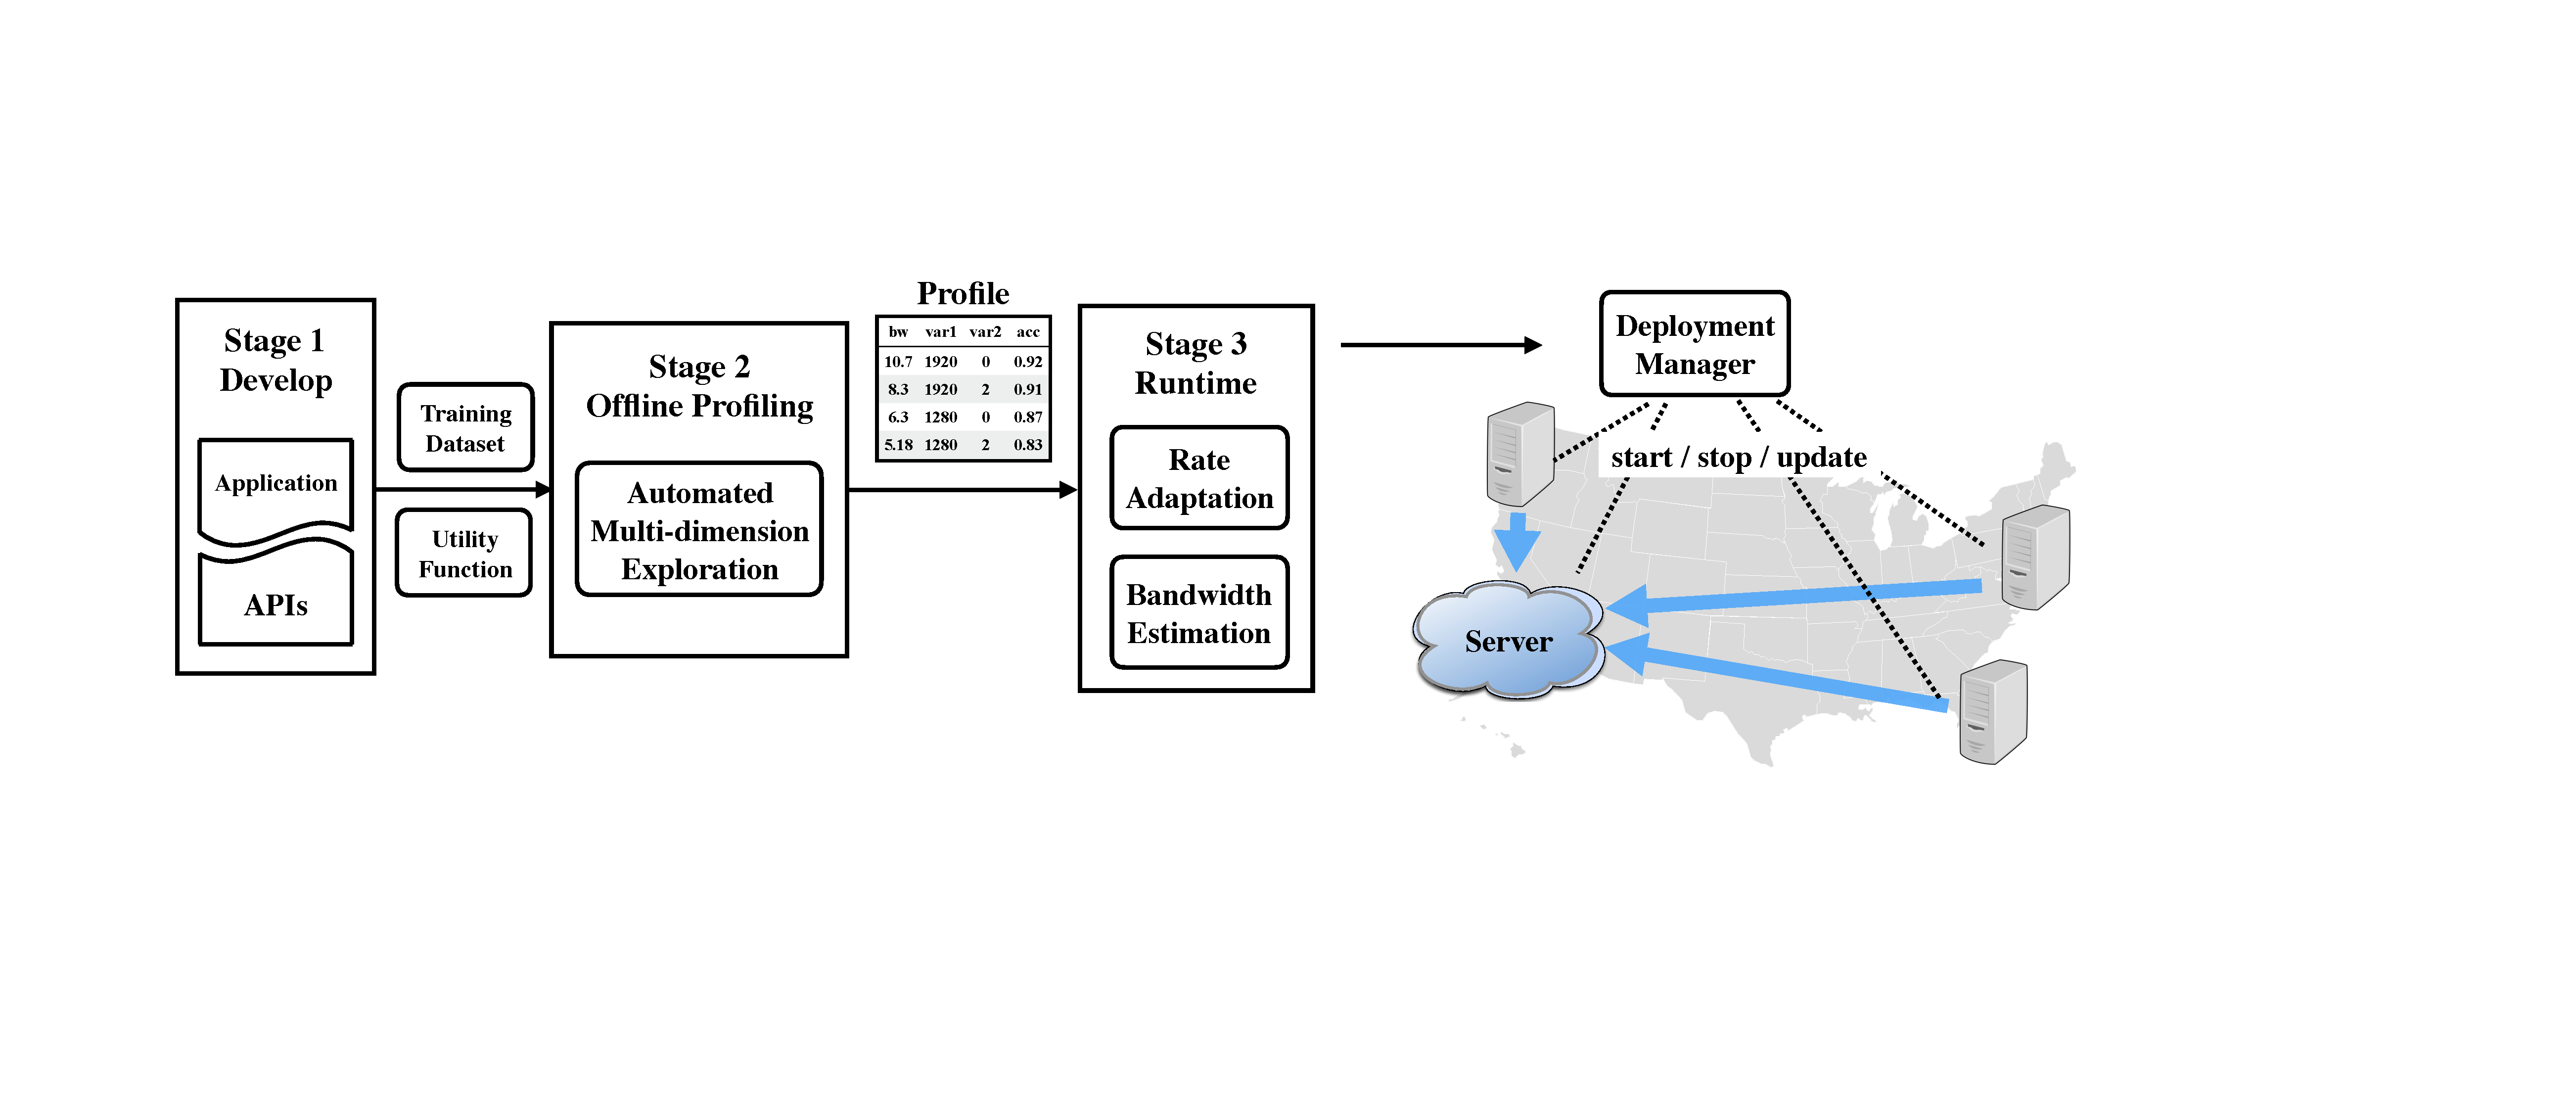
\includegraphics[width=\columnwidth]{figures/arch.pdf}
  \caption{System Overview}
  \label{fig:overview}
\end{figure}

\subsection{Programming Abstraction}
\label{sec:prog-abs}

We first consider a strawman solution: manual policies for
degradation. JetStream~\cite{rabkin2014aggregation} offers an example: ``if
bandwidth is insufficient, switch to sending images at 75\% fidelity, then 50\%
if there still isn't enough bandwidth. Beyond that point, reduce the frame rate,
but keep the images at 50\% fidelity.'' We identify the following three issues
with this approach.

\para{Lack of precision:} These policies are often developer heuristics and
rarely backed up by measurements. First, there is no direct association of the
application accuracy with the 75\% fidelity configuration. Besides, their impact
on the data size is also not trivial. Naively one would think that reducing the
frame rate by 50\% will half the data rate. However when video encoding is
employed, the inter-frame difference is increased (P-frame size) when the frame
rate is reduced. This leads to a larger data size for each
frame. \autoref{fig:h264} shows an example of H.264 encoding with four different
frame rates.

\begin{figure}
  \centering
  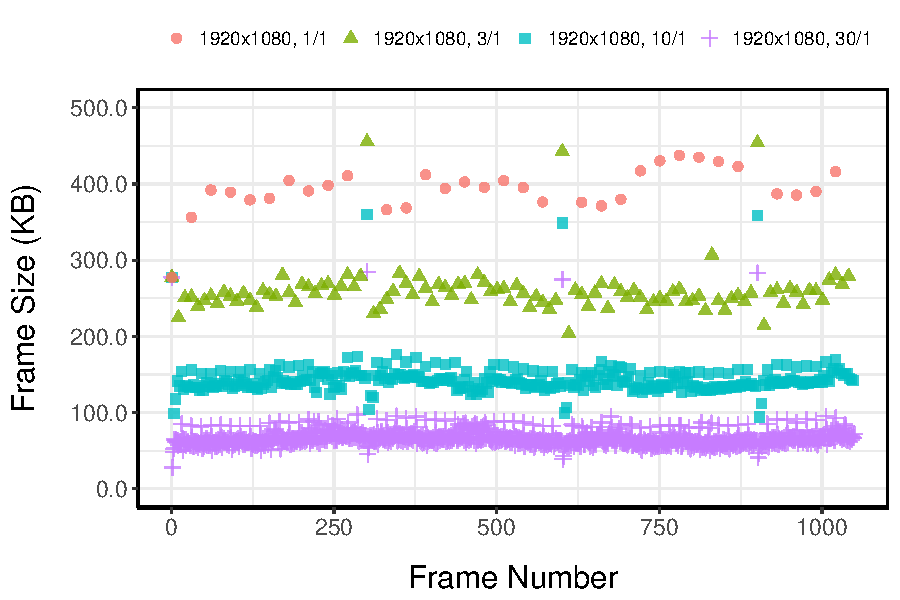
\includegraphics[width=\columnwidth]{figures/h264.pdf}
  \caption{H.264 requires more information per frame when the frame rate is
    reduced.}
  \label{fig:h264}
\end{figure}

\para{Not scalable:} The strawman solution quickly leads to too many policies
when multiple degradation operations are involved or a fine-grained control is
desired. This manual process becomes tedious and error-prone.

\para{Fixed?}

\vspace{0.5em}

The above strawman solutions clearly requires quite some developer effort to
become practical: tuning the knob to the right value and be elaborate on
individual rules.

On the other hand, a completely developer-free solution is not practical,
either. While static analysis can be used to identify places to optimize
application execution~\cite{chun2011clonecloud}, in our target applications, it
is prone to false positives---exploring wrong or unnecessary parameters. With
each introduced parameter to explore, the profiling time will increase
drastically as this poses a combinatorial space.

The ideal programming abstraction should allow explicit annotations of
degradation operations, without requiring developers being exact on the
values. Think of these APIs as hints from developers: this function, together
with these parameters, will likely reduce the data size and have an effect on
the data fidelity; however their exact effect is not clear.

With these APIs, the example we mentioned earlier can be implemented as
following.

\begin{lstlisting}
let (client, server) = adastream::network();
client.stream(Camera::new(0))
      .maybe_downsample(vec![(1600, 900), (1280, 720)])
      .maybe_skip(vec![2, 5])
      .send_to(server)
      .map(|frame| frame.show())
      .compose()
\end{lstlisting}

%%% Local Variables:
%%% mode: latex
%%% TeX-master: "sigcomm2017"
%%% End:
